\chapter{Resultados experimentales}
\label{chap:resultados}
Este capítulo presenta la evaluación del simulador desarrollado en el supercomputador Finisterrae III.
El análisis se centra en tres aspectos críticos: la parametrización eficiente de las estructuras de datos bajo restricciones de hardware, la validación de la fidelidad física del integrador y la cuantificación del rendimiento comparativo entre las arquitecturas CPU y GPU.

\section{Configuración y análisis del árbol Barnes-Hut}\label{sec:configuracion-y-analisis-del-arbol-barnes-hut}

La eficiencia del algoritmo Barnes-Hut reside en el equilibrio entre la precisión de la aproximación de fuerzas y el coste computacional asociado al recorrido de la estructura jerárquica.
La configuración del \textit{Octree} no es trivial, ya que depende intrínsecamente de la distribución de densidad del sistema estelar simulado y de las limitaciones de hardware.
Esta sección explora el espacio de parámetros críticos del algoritmo, determinando la granularidad espacial y el criterio de apertura óptimos para procesar el catálogo de Gaia DR3 sin comprometer la fidelidad física de los resultados.

\subsection{Configuración de la granularidad del árbol}\label{subsec:eleccion-de-la-granularidad-del-arbol}
La construcción del \textit{Octree} constituye el pilar fundamental del algoritmo Barnes-Hut.
La eficiencia y precisión del cálculo de fuerzas dependen de una representación jerárquica óptima, donde el parámetro \texttt{min\_subdivisions} (ver Sección~\ref{subsec:version-cpu}) desempeña un papel crítico.
Este parámetro define la granularidad del árbol: una mayor subdivisión permite una fragmentación más fina del espacio, pero incrementa exponencialmente el número de nodos y, por ende, la ocupación de memoria en el sistema.

Para determinar la viabilidad técnica en el hardware objetivo, se analizó el impacto de los niveles de subdivisión sobre la VRAM de una unidad NVIDIA A100, la cual cuenta con 40GB.
Los resultados del consumo, desglosados por cada uno de los ocho octantes principales, se presentan en la Figura~\ref{fig:vram_octantes}.

\begin{figure}[h!]
    \centering
    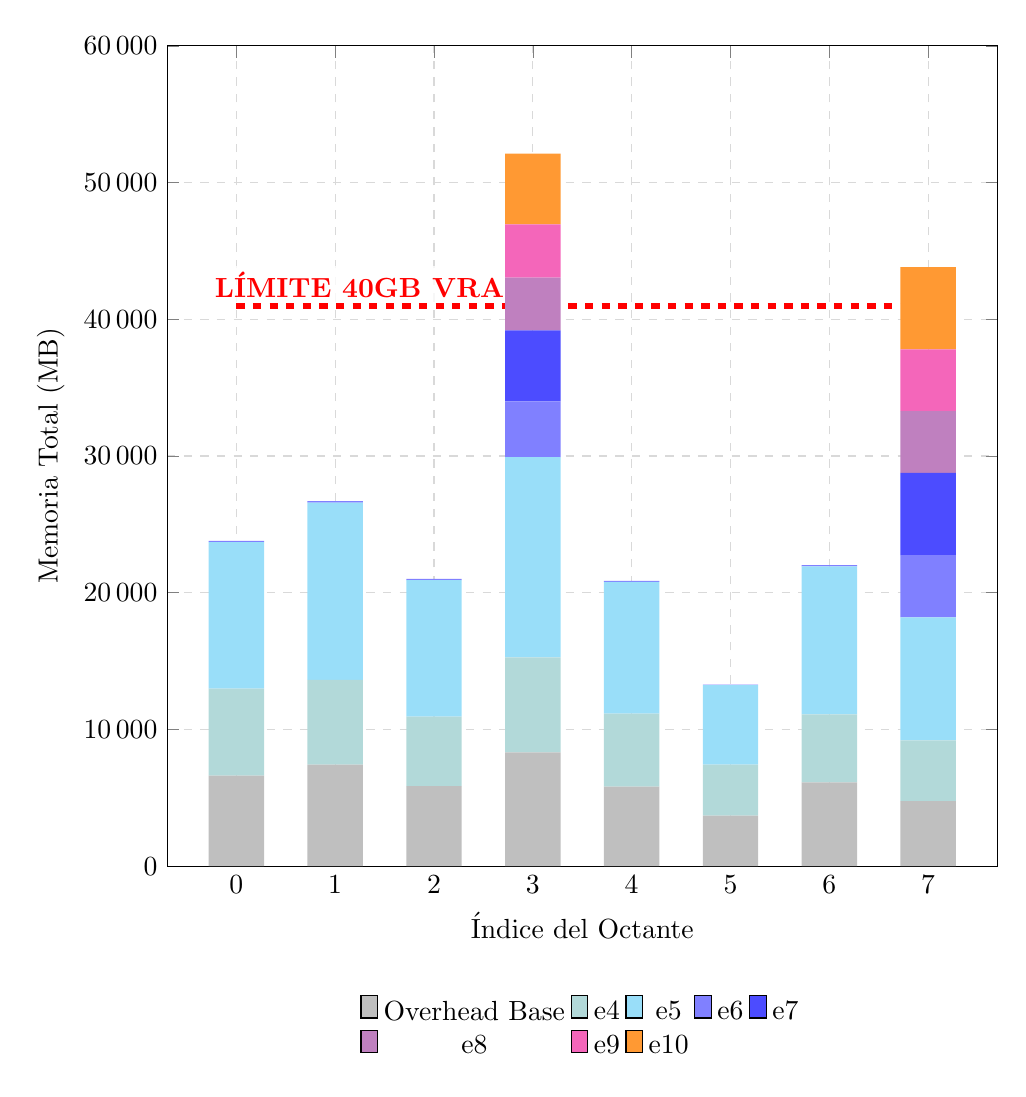
\begin{tikzpicture}
        \begin{axis}[
            ybar stacked, % Gráfico de barras apiladas
            bar width=20pt, % Ancho de las barras
            enlarge x limits=0.1, % Espacio adicional en el eje X
            width=\textwidth, height=12cm, % Dimensiones del gráfico
            ymin=0, ymax=60000, % Límites del eje Y, aumentado para evitar superposición
            ylabel={Memoria Total (MB)}, % Etiqueta del eje Y
            xlabel={Índice del Octante}, % Etiqueta del eje X
            symbolic x coords={0,1,2,3,4,5,6,7}, % Coordenadas simbólicas para el eje X
            xtick=data, % Mostrar marcas solo para los datos disponibles
            scaled y ticks=false, % Desactivar la notación científica en el eje Y
            y tick label style={/pgf/number format/fixed, /pgf/number format/1000 sep={\,}}, % Formato de etiquetas del eje Y con separador de miles
            legend style={at={(0.5,-0.15)}, anchor=north, legend columns=5, draw=none, fill=none}, % Estilo y posición de la leyenda
            grid=major, % Activar cuadrícula principal
            major grid style={dashed, gray!30} % Estilo de la cuadrícula
        ]
            % Overhead Base
            \addplot[fill=gray!50, draw=none] coordinates {(0,6622) (1,7430) (2,5851) (3,8314) (4,5813) (5,3694) (6,6131) (7,4755)};
            \addlegendentry{Overhead Base}

            % e4
            \addplot[fill=teal!30, draw=none] coordinates {(0,6359) (1,6195) (2,5085) (3,6949) (4,5340) (5,3728) (6,4979) (7,4444)};
            \addlegendentry{e4}

            % e5
            \addplot[fill=cyan!40, draw=none] coordinates {(0,10717) (1,12958) (2,9993) (3,14659) (4,9646) (5,5810) (6,10808) (7,8996)};
            \addlegendentry{e5}

            % e6
            \addplot[fill=blue!50, draw=none] coordinates {(0,89) (1,111) (2,75) (3,4074) (4,68) (5,38) (6,94) (7,4549)};
            \addlegendentry{e6}

            % e7
            \addplot[fill=blue!70, draw=none] coordinates {(0,0) (1,0) (2,0) (3,5184) (4,0) (5,0) (6,0) (7,6019)};
            \addlegendentry{e7}

            % e8
            \addplot[fill=violet!50, draw=none] coordinates {(0,0) (1,0) (2,0) (3,3867) (4,0) (5,0) (6,0) (7,4514)};
            \addlegendentry{e8}

            % e9
            \addplot[fill=magenta!60, draw=none] coordinates {(0,0) (1,0) (2,0) (3,3887) (4,0) (5,0) (6,0) (7,4515)};
            \addlegendentry{e9}

            % e10
            \addplot[fill=orange!80, draw=none] coordinates {(0,0) (1,0) (2,0) (3,5183) (4,0) (5,0) (6,0) (7,6019)};
            \addlegendentry{e10}

            \draw[red, dashed, line width=2pt] (axis cs:0,40960) -- (axis cs:7,40960)
            node[above, pos=0.2, font=\bfseries\color{red}, fill=white, fill opacity=0.8, text opacity=1, inner sep=2pt] {LÍMITE 40GB VRAM};

        \end{axis}
    \end{tikzpicture}
    \caption{Desglose de consumo de VRAM por octante según el número máximo de subdivisiones (ex se refiere a un número de subdivisiones $10^X$)}
    \label{fig:vram_octantes}
\end{figure}

En dicha figura, la categoría \textit{Overhead Base} representa el coste de memoria fijo asociado al almacenamiento de los vectores de posición y velocidad de todas las estrellas contenidas en cada octante.
Debido a que el catálogo de Gaia DR3 se distribuye de forma asimétrica, este valor varía significativamente según la población estelar de cada región.
Sobre esta base se apilan las capas correspondientes a los incrementos en \texttt{min\_subdivisions}.

Un fenómeno clave observado en el análisis es la convergencia o saturación del consumo de memoria en la mayoría de los octantes (especialmente del 0 al 2 y del 4 al 6).
Se aprecia que, a partir de $10^6$ (e6) o $10^7$ (e7) subdivisiones, el incremento de VRAM es nulo.
Este comportamiento indica que el subárbol ha alcanzado un \textbf{estado de subárbol perfecto}: la resolución espacial es tan elevada que cada estrella ha quedado aislada en su propio nodo hoja.
Una vez alcanzado este límite físico, aumentar el parámetro de subdivisión no genera nuevos nodos, ya que no existen partículas adicionales que fragmentar en dichos volúmenes de espacio.

A diferencia de estas regiones, los octantes 3 y 7 —correspondientes al plano galáctico y al núcleo de la Vía Láctea— presentan un crecimiento sostenido debido a su altísima densidad estelar.
En estas zonas, el \textit{Octree} requiere niveles de profundidad muy superiores para lograr el aislamiento de las partículas.
Este fenómeno justifica la elección de \textbf{$10^7$} como valor para \texttt{min\_subdivisions}.
Bajo esta configuración, el octante 3 alcanza una ocupación cercana a los 39.180 MB, operando en el umbral crítico de la capacidad de la NVIDIA A100.
Elevar la granularidad a $10^8$ resultaría en un consumo proyectado superior a los 43 GB en los octantes densos, lo que excedería la VRAM disponible y provocaría el colapso de la simulación por errores de tipo \textit{Out of Memory} (OOM).
Mientras que la GPU está sujeta a restricciones de memoria segmentada por octante, la versión CPU solo se ve limitada por el consumo global de RAM.
No obstante, se ha decidido igualar la granularidad en CPU al techo impuesto por el hardware gráfico para asegurar que cualquier divergencia en los resultados se deba exclusivamente a la arquitectura de cómputo y no a una disparidad en la resolución estructural del árbol.

Para la configuración final con $10^7$ subdivisiones ($e^7$), la construcción resultó en una estructura masiva de \textbf{1.834.641.228 nodos}, requiriendo un total de \textbf{146.970 MB} de memoria para el árbol completo.

\subsection{Elección del parámetro Theta}\label{subsec:eleccion-parametro-theta-theta}

El parámetro de apertura $\theta$ constituye la variable de control crítica en el algoritmo Barnes-Hut, determinando el umbral a partir del cual un nodo interno del \textit{octree} puede ser tratado como una única superpartícula (aproximación multipolar) en lugar de evaluar sus constituyentes individuales.
En simulaciones cosmológicas estándar de baja densidad, es habitual adoptar valores de $\theta \approx 0.5$ o incluso superiores para maximizar el rendimiento.
Sin embargo, el presente estudio modela un sistema extremadamente compacto ($N \approx 1,1 \times 10^9$ estrellas) con un radio de giro efectivo de $R_g \approx 3,86$ kpc, lo que resulta en densidades volumétricas superiores a $4,5 \times 10^6$ estrellas/kpc$^3$.

En un sistema tan compacto, la fuerza de gravedad cambia muy bruscamente en distancias cortas (altos gradientes).
Si se elige un valor de $\theta$ demasiado alto, el algoritmo agruparía grandes cantidades de estrellas en un solo centro de masa demasiado pronto.
Esto provocaría una pérdida de resolución en el cálculo de fuerzas, suavizando artificialmente la gravedad real en el núcleo.
Como consecuencia, las estructuras finas, como cúmulos estelares, podrían desintegrarse erróneamente, y las estrellas ganarían velocidad de forma artificial (calentamiento dinámico) debido a errores numéricos, alterando la evolución real de la galaxia.

Para determinar el valor óptimo, se realizó un análisis de convergencia empleando una submuestra aleatoria de 10.000 estrellas.
La metodología experimental consiste en calcular el vector de aceleración gravitatoria que experimenta cada estrella de esta muestra debido a la influencia de la galaxia completa (1.100 millones de cuerpos).
Para ello, se genera una solución de referencia exacta mediante fuerza bruta (sumatorio directo de todas las interacciones par a par) y se confronta con la aproximación obtenida por el algoritmo Barnes-Hut para distintos valores de $\theta$.
Esta comparativa permite cuantificar simultáneamente la discrepancia vectorial (error relativo en la aceleración) y la ganancia en velocidad de procesamiento (\textit{speedup}).

La razón de usar un subconjunto de prueba es poder usar la aproximación de fuerza bruta como --ground truth--.
El conjunto de prueba escogido es estadísticamente representativo de la población total, ya que el muestreo cubre uniformemente tanto las regiones de altísima densidad del bulbo como la periferia dispersa.
La baja desviación estándar observada en los resultados confirma que esta muestra captura fielmente la varianza del error del algoritmo, permitiendo extrapolar el comportamiento del sistema completo sin incurrir en el coste computacional prohibitivo de evaluar la totalidad del catálogo para cada punto de prueba.

Los resultados, mostrados en la Figura~\ref{fig:theta}, dictan la elección de \textbf{$\theta = 0,2$} basándose en tres criterios fundamentales:

\begin{enumerate}
    \item \textbf{Acotación del Error Máximo:} Mientras que el error medio tiende a diluir los casos extremos, el error máximo ($L_\infty$) revela la estabilidad en las peores configuraciones geométricas. Para $\theta = 0,2$, el error máximo se mantiene en un 0,13\%. Al incrementar $\theta$ a 0,5, este error se dispara al 2,5\%, un nivel inaceptable que podría expulsar estrellas de sus órbitas en el denso bulbo galáctico.

    \item \textbf{Impacto en la Evolución Dinámica:} Traduciendo el error relativo medio obtenido ($4,14 \times 10^{-5}$) a magnitudes físicas, la incertidumbre en la aceleración para una estrella típica del bulbo ($a \approx 0,01$ kpc/Myr$^2$) es del orden de $4 \times 10^{-7}$ kpc/Myr$^2$. En una integración temporal de 100 Myr, esto induce una deriva de posición ($\Delta x$) de aproximadamente:
    \begin{equation}
        \Delta x \approx \frac{1}{2} a_{err} t^2 \approx 2 \text{ parsecs}
    \end{equation}
    Esta desviación de \textbf{2 parsecs} es despreciable frente a la escala del sistema ($R_g \approx 3860$ pc), garantizando la estabilidad orbital a largo plazo.
    En contraste, un valor de $\theta=0,5$ implicaría derivas cercanas a los 300 pc, lo que comprometería la resolución de las estructuras finas del núcleo.

    \item \textbf{Conservación de Energía:} La precisión de $10^{-5}$ asegura que la interacción gravitatoria se calcule con una fidelidad cercana a la aritmética de doble precisión, minimizando la fricción numérica y preservando la energía total del sistema sin necesidad de recurrir a la fuerza bruta.
\end{enumerate}

En conclusión, se ha seleccionado $\theta = 0,2$ como un parámetro de Alta Fidelidad.
Aunque esta configuración es computacionalmente más exigente que los estándares habituales reduciendo el \textit{speedup} potencial de $\sim 2000$x a $\sim 470$x, es la única que garantiza que la evolución morfológica de la galaxia simulada responda a leyes físicas reales y no a artefactos de la aproximación algorítmica.

\begin{figure}[h!]
    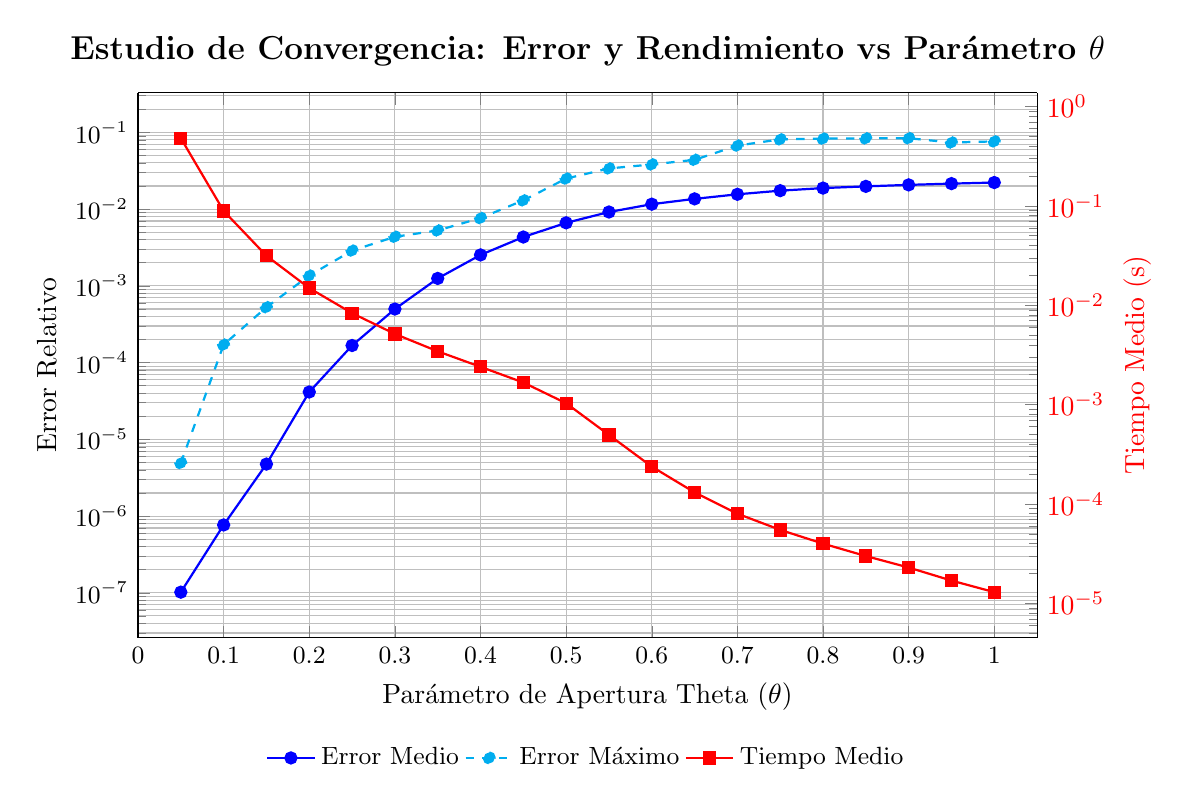
\begin{tikzpicture}
        \begin{axis}
            [
            width=13cm, height=8.5cm,
            title={Estudio de Convergencia: Error y Rendimiento vs Parámetro $\theta$},
            xlabel={Parámetro de Apertura Theta ($\theta$)},
            ylabel={Error Relativo},
            ymode=log,
            axis y line*=left,
            grid=both,
            xmin=0, xmax=1.05,
            xtick={0,0.1,0.2,0.3,0.4,0.5,0.6,0.7,0.8,0.9,1.0},
            % --- LEYENDA UNIFICADA ---
            legend style={
                at={(0.5,-0.18)},
                anchor=north,
                legend columns=3,
                draw=none,
                font=\small
            },
            tick label style={font=\small},
            title style={font=\large\bfseries}
                ]
                % 1. Error Medio (Azul, Círculo)
                \addplot[color=blue, mark=*, thick] coordinates {
                (0.05, 1.02e-07) (0.10, 7.66e-07) (0.15, 4.76e-06) (0.20, 4.14e-05)
                (0.25, 1.67e-04) (0.30, 4.99e-04) (0.35, 1.25e-03) (0.40, 2.53e-03)
                (0.45, 4.33e-03) (0.50, 6.63e-03) (0.55, 9.17e-03) (0.60, 1.16e-02)
                (0.65, 1.36e-02) (0.70, 1.56e-02) (0.75, 1.74e-02) (0.80, 1.88e-02)
                (0.85, 1.98e-02) (0.90, 2.07e-02) (0.95, 2.15e-02) (1.00, 2.22e-02)
            };
                \addlegendentry{Error Medio}

                % 2. Error Máximo (Cian, Cruz)
                \addplot[color=cyan, mark=*, dashed, thick] coordinates {
                (0.05, 4.91e-06) (0.10, 1.71e-04) (0.15, 5.27e-04) (0.20, 1.36e-03)
                (0.25, 2.88e-03) (0.30, 4.36e-03) (0.35, 5.27e-03) (0.40, 7.65e-03)
                (0.45, 1.30e-02) (0.50, 2.50e-02) (0.55, 3.39e-02) (0.60, 3.82e-02)
                (0.65, 4.39e-02) (0.70, 6.73e-02) (0.75, 8.11e-02) (0.80, 8.29e-02)
                (0.85, 8.35e-02) (0.90, 8.40e-02) (0.95, 7.37e-02) (1.00, 7.63e-02)
            };
                \addlegendentry{Error Máximo}

                % 3. Entrada manual para el Tiempo Medio (Rojo, Cuadrado)
                \addlegendimage{color=red, mark=square*, thick}
                \addlegendentry{Tiempo Medio}

        \end{axis}

        % Segundo eje para el Tiempo
        \begin{axis}[
            width=13cm, height=8.5cm,
            axis y line*=right,
            axis x line=none,
            ymode=log,
            ylabel={Tiempo Medio (s)},
            ylabel style={red},
            yticklabel style={red},
            xmin=0, xmax=1.05
        ]
            \addplot[color=red, mark=square*, thick] coordinates {
                (0.05, 0.478950) (0.10, 0.088903) (0.15, 0.031436) (0.20, 0.014875)
                (0.25, 0.008326) (0.30, 0.005144) (0.35, 0.003440) (0.40, 0.002401)
                (0.45, 0.001671) (0.50, 0.001033) (0.55, 0.000496) (0.60, 0.000238)
                (0.65, 0.000131) (0.70, 0.000080) (0.75, 0.000055) (0.80, 0.000040)
                (0.85, 0.000030) (0.90, 0.000023) (0.95, 0.000017) (1.00, 0.000013)
            };
        \end{axis}
    \end{tikzpicture}
    \caption{Gráfica de resultados parámetro theta}
    \label{fig:theta}
\end{figure}

\section{Validación del integrador Leapfrog}\label{sec:precision-fisica-y-validacion-del-integrador-leapfrog}

Para garantizar la integridad científica del simulador antes de proceder con ejecuciones de larga duración, se implementaron tests de validación jerárquica.
Esta metodología permite aislar errores en las constantes físicas, la lógica del integrador temporal y las aproximaciones algorítmicas del Octree.

\subsection{Estabilidad del potencial y constantes (Test Unitario)}

En primer lugar, se validó la implementación de las aceleraciones analíticas (Halo NFW y Bulbo de Hernquist) y el esquema de integración \textit{Leapfrog Kick-Drift-Kick}.
Para ello, se situó una estrella de prueba a una distancia de $8,2$~kpc del centro galáctico.
La velocidad inicial se derivó analíticamente a partir del potencial calculado por el motor de física para forzar una órbita circular teórica ($\approx 151,85$~km/s).

Tras una evolución equivalente a $100$~Myr, el radio orbital se mantuvo constante en $8,2000$~kpc.
La ausencia de deriva radial confirma que las constantes físicas ($G$ y parámetros de escala) están correctamente dimensionadas y que el integrador es capaz de mantener órbitas estables en potenciales conservativos.

\subsection{Integridad del pipeline de datos (Stress-test Analítico)}

Con el objetivo de validar la robustez del sistema ante el volumen real de datos de Gaia ($N \approx 1,1 \times 10^9$), se realizó una prueba de integración masiva desactivando las fuerzas estrella-estrella.
Este test evalúa la estabilidad de los bucles de computación paralela y la gestión de memoria sin el ruido introducido por las aproximaciones del árbol.

El sistema demostró una capacidad de procesamiento de \textbf{1.067,94 millones de estrellas por segundo} utilizando 64 hilos en la versión CPU.
El éxito de este test garantiza que el \textit{pipeline} de actualización de posiciones y velocidades es determinista y está libre de condiciones de carrera (\textit{race conditions}) para este volumen de datos.

\subsection{Reversibilidad y simetría algorítmica (Test de Leapfrog)}

La validación definitiva del algoritmo de Barnes-Hut se realizó mediante un test de reversibilidad temporal utilizando una submuestra estadísticamente representativa del 1\% del catálogo (10,6 millones de estrellas) con masas escaladas.
El uso de esta muestra reducida es fundamental desde el punto de vista operativo, ya que realizar una prueba de reversibilidad de cuatro pasos con el dataset completo requeriría una gran reserva de recursos en el supercomputador durante demasiado tiempo, conllevando colas sustanciales incompatibles con los plazos de entrega del proyecto.
Esta prueba aprovecha la naturaleza simpléctica del integrador \textit{Leapfrog}, la cual dicta que, en ausencia de errores numéricos, el sistema debe regresar a su estado inicial si se invierte el sentido del tiempo.

Los resultados obtenidos tras evolucionar el sistema varios pasos hacia adelante y hacia atrás muestran un error medio absoluto (MAE) de \textbf{$5,20 \times 10^{-17}$~kpc}.
Este valor, situado en el límite de la precisión de doble punto flotante de la arquitectura (\textit{machine epsilon}), demuestra que la construcción del Octree y el cálculo de fuerzas son perfectamente simétricos y que el esquema de integración preserva la información del espacio de fase de manera excepcional.

\subsection{Conservación del Momento Angular}

Finalmente, se analizó la estabilidad del momento angular total en el eje de rotación galáctico ($L_z$). En un sistema aislado, esta magnitud debe permanecer constante por simetría rotacional.
Utilizando la muestra reducida, se observó una variación relativa de $L_z$ de tan solo \textbf{$1,96 \times 10^{-8}$} tras cinco pasos de simulación.

Esta mínima deriva confirma que las aproximaciones introducidas por el criterio de apertura de Barnes-Hut no introducen torques ficticios significativos.
La galaxia simulada conserva su estructura rotacional, validando la fidelidad del algoritmo para estudios de dispersión estelar a escalas de tiempo galácticas.

\section{Evaluación del simulador paralelo}\label{sec:evaluacion-de-rendimiento-y-precision-cpu-vs-gpu}

En esta sección se presenta un análisis exhaustivo del rendimiento computacional y la fidelidad física del sistema paralelo propuesto.
El objetivo es cuantificar la aceleración obtenida mediante infraestructuras HPC y validar que la paralelización masiva en GPU preserva la integridad científica frente a la ejecución de referencia en CPU.

\subsection{Análisis del rendimiento}\label{subsec:analisis-de-escalabilidad-y-computo-multi-gpu}

El cálculo de interacciones gravitatorias en un sistema de $N \approx 10^9$ estrellas constituye un reto de escala exa-escalar.
Para establecer una línea base de eficiencia, se han realizado pruebas de perfilado unitario en el supercomputador \textbf{Finisterrae III}:

\begin{itemize}
    \item \textbf{Referencia (Fuerza Bruta $O(N^2)$):} La evaluación secuencial directa de la Ley de Gravitación Universal arroja un tiempo medio de \textbf{6.987946 segundos por estrella}, por lo que completar la simulación de un solo paso temporal para la muestra requeriría aproximadamente \textbf{235 años}, lo que ilustra la inviabilidad absoluta de este enfoque.
    \item \textbf{Barnes-Hut Secuencial ($O(N \log N)$):} La aplicación del algoritmo de árbol optimiza el tiempo a \textbf{0.0148 segundos por estrella}. En un solo hilo de CPU, el tiempo estimado para la simulación de un único paso temporal se reduce a \textbf{183 días}, una mejora crítica pero insuficiente para simulaciones evolutivas con un número elevado de pasos temporales.
\end{itemize}
La versión paralela con OpenMP ejecutada en un nodo del Finisterrae III utilizando 64 núcleos reduce el tiempo de ejecución a unas 60 horas, lo que supone una aceleración de aproximadamente 70x.
Este fenómeno, conocido como \textbf{aceleración superlineal} (rendimiento superior al número de núcleos empleados), se atribuye principalmente a dos factores arquitectónicos:
\begin{enumerate}
    \item \textbf{Efecto de agregación de caché:} En la ejecución secuencial, el volumen masivo de datos de los 1.100 millones de estrellas desborda la capacidad de la memoria caché del procesador, forzando accesos continuos a la memoria RAM principal.
    Al distribuir la carga entre 64 núcleos, el subconjunto de datos que maneja cada hilo es considerablemente menor, permitiendo que una mayor proporción de estos datos resida en las memorias caché locales de cada núcleo, reduciendo drásticamente la latencia de acceso.
    \item \textbf{Ancho de banda de memoria agregado (Dual-Socket):} Los nodos de computación del Finisterrae III emplean una arquitectura dual-socket, integrando dos CPUs físicas independientes en la misma placa base.
    En una ejecución secuencial, el proceso queda confinado a un único zócalo, limitado por los canales de memoria de ese procesador específico.
    Sin embargo, al utilizar los 64 núcleos simultáneamente, se activan los controladores de memoria de ambas CPUs.
    Esto permite explotar el ancho de banda agregado de todo el nodo, duplicando la capacidad efectiva de transferencia de datos desde la RAM y eliminando cuellos de botella que saturaban al hilo único.
\end{enumerate}

Aunque la verdadera capacidad del sistema se manifiesta al aplicar paralelismo masivo mediante CUDA. Se ha evaluado el tiempo de ejecución de un paso completo de simulación en el nodo \texttt{a100-m8} (nodo del Finisterrae III que dispone de ocho GPUs A100), comparando la ejecución multihilo en CPU (64 núcleos con OpenMP) frente a una configuración de hasta ocho GPUs NVIDIA A100.
Es importante señalar que las métricas presentadas no corresponden a una ejecución aislada.
Dado que el sistema de archivos paralelo Lustre es un recurso compartido con carga de trabajo variable, los tiempos de entrada/salida pueden sufrir fluctuaciones.
Por ello, los valores corresponden a la media aritmética de múltiples iteraciones, procedimiento adoptado para mitigar el ruido introducido por la latencia del sistema de archivos y ofrecer una estimación robusta.

Los resultados de este análisis se presentan a continuación: la Tabla~\ref{tab:rendimiento_gpu} detalla la escalabilidad y aceleración global del sistema, mientras que la Tabla~\ref{tab:comparativa_cpu_gpu} ofrece un desglose de los tiempos invertidos en cada etapa del algoritmo.

\begin{table}[htbp]
    \centering
    % X: columna auto-ajustable, c: columna centrada
    \begin{tabularx}{\textwidth}{|X|c|c|}
        \hline
        \textbf{Etapa del Algoritmo} & \textbf{CPU} & \textbf{8 GPUs} \\ \hline

        % \multicolumn{columnas}{alineacion}{texto}
        Lectura de datos & \multicolumn{2}{c|}{59.12 s} \\ \hline

        Construcción del árbol  & 442.32 s & 111.73 s \\ \hline
        Cálculo de Aceleraciones y KDK  & 29 h 46 min & 12 min 24 s \\ \hline
        Escritura de resultados & \multicolumn{2}{c|}{36.39 s} \\ \hline
        \textbf{Tiempo Total} & \textbf{59:42:29} & \textbf{00:28:16} \\ \hline
    \end{tabularx}
    \caption{Comparativa de tiempos de ejecución desglosados por etapas}
    \label{tab:comparativa_cpu_gpu}
\end{table}

\begin{table}[H]
    \centering
    \begin{tabular}{|c|c|c|}
        \hline
        \textbf{Hardware} & \textbf{Tiempo (HH:MM:SS)} & \textbf{Aceleración (\textit{Speedup})} \\ \hline
        CPU (64 núcleos)  & 59:42:29                   & 1,0x (Referencia)                       \\ \hline
        1 GPU             & 02:20:23                   & 25,5x                                   \\ \hline
        2 GPUs            & 01:24:49                   & 42,2x                                   \\ \hline
        3 GPUs            & 01:06:12                   & 54,1x                                   \\ \hline
        4 GPUs            & 00:46:32                   & 76,9x                                   \\ \hline
        5 GPUs            & 00:47:56                   & 74,7x                                   \\ \hline
        6 GPUs            & 00:48:13                   & 74,3x                                   \\ \hline
        7 GPUs            & 00:42:19                   & 84,6x                                   \\ \hline
        \textbf{8 GPUs}   & \textbf{00:28:16}          & \textbf{126,7x}                         \\ \hline
    \end{tabular}
    \caption{Tiempos de ejecución y escalabilidad en el nodo \texttt{a100-m8} frente a la solución en CPU}
    \label{tab:rendimiento_gpu}
\end{table}

El análisis revela un \textit{speedup} de \textbf{126.7x} al utilizar la capacidad total del nodo.
La aceleración conseguida con respecto al sistema secuencial es de más de 9000x, consiguiendo una reducción del tiempo de pared de casi \textbf{183 días a tan solo 28 minutos}, lo que transforma un problema prohibitivo en un flujo de trabajo manejable.

En cuanto a la escalabilidad del sistema, se aprecia un comportamiento lineal altamente eficiente hasta el uso de cuatro GPUs.
No obstante, en el intervalo comprendido entre las cuatro y siete unidades de procesamiento el rendimiento muestra una meseta técnica atribuible a la propia arquitectura del algoritmo de descomposición espacial.
Dado que el nivel superior del árbol se divide en exactamente ocho octantes, las configuraciones que no son submúltiplos exactos de este número incurren en un desequilibrio de carga.
Específicamente, con cuatro a siete GPUs, el sistema se ve obligado a realizar al menos dos iteraciones de cálculo en algunas unidades para cubrir la totalidad de los octantes, provocando que ciertos núcleos permanezcan ociosos mientras otros completan su segundo ciclo de procesamiento.
Este cuello de botella desaparece al alcanzar las ocho GPUs, donde la correspondencia uno a uno entre octantes y unidades de procesamiento permite una ocupación del hardware del 100\%.

\subsection{Validación de la precisión numérica y estabilidad física}\label{subsec:validacion-de-la-precision-numerica-y-estabilidad-fisica}

La migración de algoritmos de simulación de N-cuerpos a arquitecturas GPU introduce desafíos inherentes a la precisión numérica.
Debido a que la aritmética de coma flotante no es asociativa bajo el estándar \textit{IEEE 754}, el orden de las operaciones en los hilos de ejecución de CUDA altera los bits menos significativos del resultado.
En un algoritmo de Barnes-Hut, estas pequeñas diferencias pueden provocar que la CPU y la GPU tomen decisiones ligeramente distintas sobre la apertura de nodos del \textit{octree}, magnificando la divergencia.

\subsubsection{Análisis del error y bits efectivos}
El error medio absoluto (MAE) en posición tras el primer paso es de $6.4460 \times 10^{-5}$ kpc.
Para cuantificar la fidelidad del cálculo frente a la escala global del sistema, se ha calculado la cantidad de \textbf{bits efectivos} de precisión mediante la relación logarítmica entre la mediana del error y el radio de giro del sistema ($R_g \approx 3.86$ kpc):

\begin{equation}
    \text{Bits}_{eff} = -\log_{2} \left( \frac{\text{Mediana}(\text{Error})}{R_g} \right) \approx 15.90 \text{ bits}
\end{equation}

Este valor de \textbf{15.90 bits} indica que la CPU y la GPU mantienen una concordancia binaria en los 16 bits más significativos de la mantisa.
Si bien la integración cinemática (posiciones y velocidades) se realiza en precisión doble (\texttt{double}), el cálculo de fuerzas depende de las masas y la geometría de los nodos del árbol, almacenados en precisión simple (\texttt{float}, mantisa de 23 bits) para optimizar el uso de memoria.
Por tanto, una retención de casi 16 bits tras billones de interacciones paralelas representa un resultado robusto, ya que la precisión global del sistema está acotada superiormente por los datos en coma flotante de simple precisión.
En términos decimales, esto equivale a una precisión de aproximadamente cinco dígitos significativos de concordancia absoluta.

\subsubsection{Estabilidad y conservación del momento}
La métrica más crítica para la validez física es la deriva del centro de masas (\textit{CoM Drift}). Se ha registrado un desplazamiento residual de $1.1656 \times 10^{-06}$ kpc.

\begin{equation}
    \Delta \vec{R}_{CoM} = \left| \frac{\sum m_i \vec{x}_{i,GPU}}{\sum m_i} - \frac{\sum m_i \vec{x}_{i,CPU}}{\sum m_i} \right|
\end{equation}

Al ser este valor cuatro órdenes de magnitud inferior al error de posición individual y despreciable frente al radio del sistema, se confirma que las asimetrías numéricas de la GPU no introducen sesgos físicos artificiales.
El sistema preserva la conservación del momento lineal, garantizando que la evolución de la estructura galáctica a gran escala sea físicamente equivalente a la obtenida en CPU.


En conclusión, el sistema desarrollado no solo ofrece una aceleración de órdenes de magnitud respecto a la versión secuencial, sino que mantiene una fidelidad numérica que garantiza la producción de resultados científicos robustos en el supercomputador Finisterrae III.